\documentclass[notitlepage]{report}   % list options between brackets
%\usepackage{}              % list packages between braces
\usepackage{epsfig}
\usepackage{graphicx}
\usepackage{amsfonts}
\usepackage{enumerate}
\usepackage{dsfont}
\usepackage{amsmath}

	
% type user-defined commands here

\begin{document}

	\title{Introduction to Statistical Learning}  

	\author{
      {D\'{e}partement de Math\'{e}matique}\\
		{ENS Cachan}\\
		{Cachan, Paris}\\
		\\
		Prof. Nicolas VAYATIS
	}
	\date{Fall 2012}  
	\maketitle

	\begin{abstract}
      These notes contain the contents of the course to ``Introduction to Statistical Learning''. It covers the mathematical basis for supervised learning modelling and discusses classification algorithms for handling high-dimensional problems.

	\end{abstract}

	\tableofcontents

	\chapter{Performance and optimization issues.}

	\section{Introduction.}

		Assume two data sets, as depicted in 
		Figures~\ref{fig:chap1_scatters}. Each data set has two known classes, 
		represented by circles and x marks. Consider that we are interested in 
		classifying new-observations of unknown data, represented by black bullet 
		marks, in either circles and x marks class. 
      Empirically, we may conclude that a given observation belong to the class 
		of the known  data, whose it has the \emph{closest relation}. However, 
      in same cases,  we might mislead the  classification of black bullets if the 
		relation between known and unknown data is not clear or poorly defined. 
      In order to address this issue, statistical learning provides methods 
		for modelling classification problems properly. These methods allows us to 
		define the performance targets, to grasp the main patterns from the known data, 
		and to handle the classification error.

		\begin{figure}
			\centering
			\begin{tabular}{l@{}l@{}}
		 		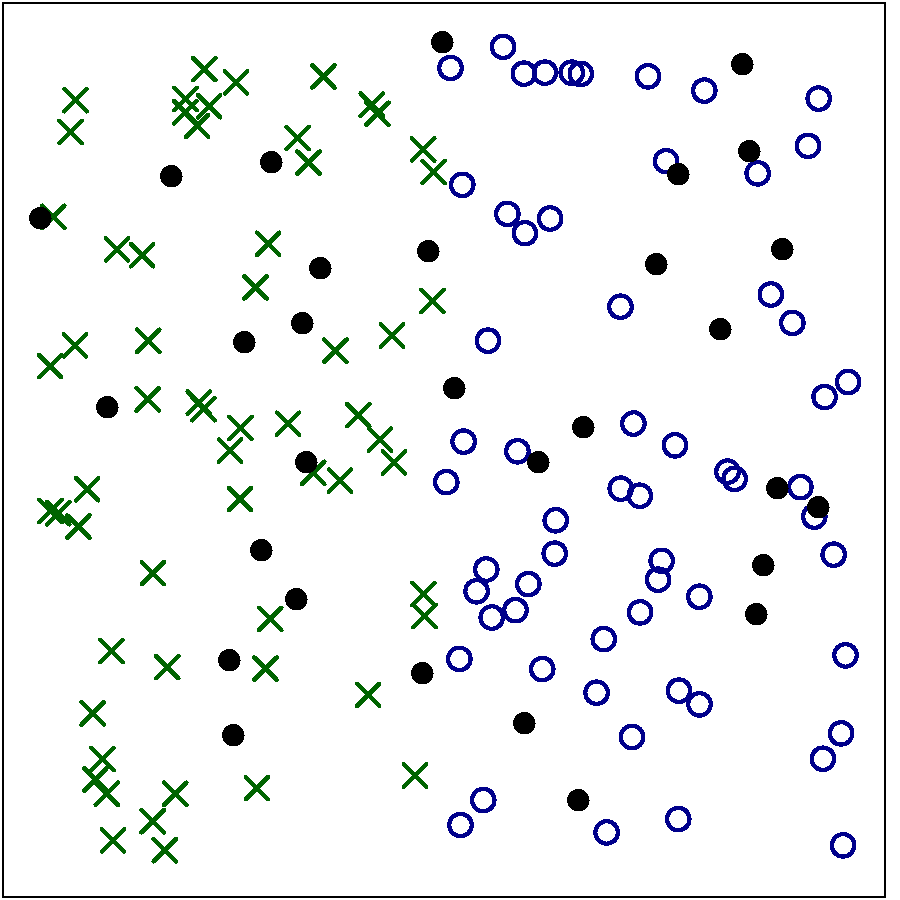
\includegraphics[width=0.45\textwidth]{inputs/img/chap1_scatter_intro_ds1} &
				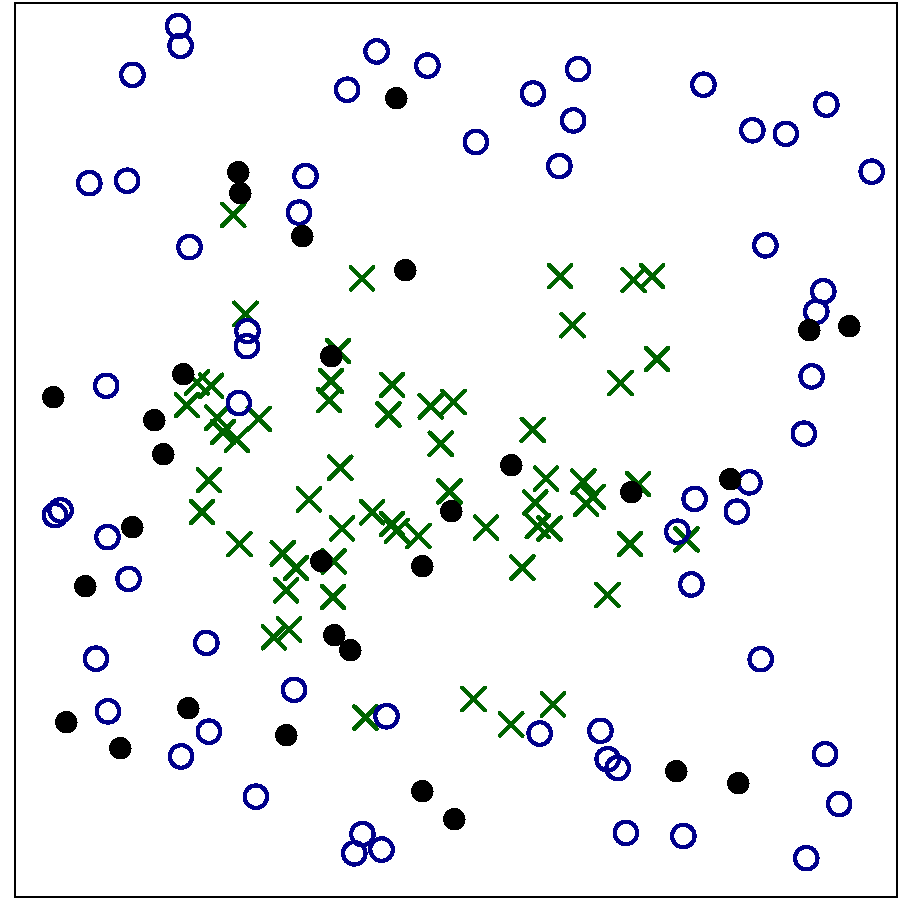
\includegraphics[width=0.45\textwidth]{inputs/img/chap1_scatter_intro_ds2} \\
			\end{tabular}
			\caption{Two classification examples in two dimensions. There are two known classes, circles and x marks. The problem is to classify the the unknown data, black bullets, into one of the two classes.}
		  	\label{fig:chap1_scatters}
		\end{figure}


	\section{Probabilistic model for data.}

		In this section we present our basic model. 
		
		In general, we define the law of $(X{\times}Y)$ as

		\begin{equation}
			(X,Y) \sim \mathbb{P}.
			\label{x_y_law}
		\end{equation}

		Assuming $x \in \mathcal{X}$, we can state that,

		\begin{equation}
			\mathcal{X} = \mathcal{R}^d.
			\label{x_example}
		\end{equation}

		where observations are represented by $d$-dimensional vector $x$. 

		In supervised learning, $y$ exists. It denotes the unknown nature of the observation, 
		and its characteristics depends on the classification problem. For instance,

		\begin{itemize}
			\item $|y|=2$, a binary problem, e.g. $Y = \{0,1\} \mbox{ or } \{-1,1\}.$;
			\item $|y|=K$, classification in a finite set of size K ;
			\item $y \doteq \mathbb{R}$, regression;
			\item $y = \mathbb{R}^K$, multi-task;
			\item $|y| = K$ observing the relative ordering between different values of $y$, ordinal regression.
		\end{itemize}
		
		\subsection{Definition of the law of $\mathbb{P}$.}

			We present two definitions of $\mathbb{P}$:

			\begin{enumerate}[a)] % a), b), c), ...
				\item Generative definition.
					\begin{equation}
						\mathcal{L}(X,Y) \equiv \mathbb{P} \leftrightarrow (\mathcal{Y}(Y), \mathcal{Y}(X|Y)).
						\label{p_generative_law_example}
					\end{equation}
				e.g. for $y=\{-1,+1\}$\\ 
				\centerline{$\mathcal{L}(X|Y) \leadsto (\mathbb{P}_{+},\mathbb{P}_{-})$}

				considering $\mathcal{L}(X|Y) \leadsto \mathcal{L}(X)$, and $(\mathbb{P}_{+},\mathbb{P}_{-}) \leadsto \mathcal{Y}(X|Y_{=+1})$, we have\\ 
				\centerline{$\mathbb{P}_X = _{P}\mathbb{P}_{+} + _{1-P}\mathbb{P}_{-}$}


				\item Alternative definition through a \emph{posteriori probability} function \cite{tc_Lugosi} (so-called ``dissertatif'' in french).
					\begin{equation}
						\mathcal{Y}(X,Y) \equiv (\mathcal{L}(X)\mathcal{L}(Y|X)).
						\label{p_generative_law_example}
					\end{equation}
			\end{enumerate}
			so that\\
			\centerline{$\forall x \in, \eta(x)=\mathbb{P}(Y=1|X=-1)$}
			Here, $\eta(x)$ represents the state of $X$.
		


	\section{Prediction problem statement.}
		
		\subsection{Types of prediction problems.}
			Based on the learning scenario, we can list predictions problems as follows:
	
			\begin{itemize}
				\item Classification: 
					\begin{itemize}
						\item classification data: $|y|<+\infty$; 
						\item goal: predict a new $x$.
					\end{itemize}
				\item Scoring or bipartite raking: 
					\begin{itemize}
						\item classification data: $|y|<+\infty$; 
						\item goal: ordering a new bunch of $X$, $(x_1,x_2,\dots,x_m)$, taking into account the state of $x$, where $\eta(x)=\mathbb{P}(Y=1|X=x)$. An remarkable example of this kind of problem is the ranking mechanism of search engines.
					\end{itemize}
				\item Raking: 
					\begin{itemize}
						\item data features: e.g. $|y|=\{1,2,3\}$, where $1 \ll 2 \ll 3$;
						\item goal: ordering a new bunch $x$.
					\end{itemize}
				\item Preference learning: 
					\begin{itemize}
							\item $(X,X')$, and $sign(y-y')$
						\item goal: binary classification $(X,X'_Z)$, where $Z \in \{-1,1\}$.
					\end{itemize}
			\end{itemize}

		\subsection{How to approach a prediction problem.}
			\begin{itemize}
				\item Define the performance goal $R$. 
				\item Select the set of predictors $\mathcal{F}$. Examples: 
					\begin{itemize}
							\item Binary classification: $\mathnormal{f}:\mathbb{R}^d\rightarrow\{-1,1\}$
							\item Scoring: $\mathnormal{f}:\mathbb{R}^d \times \dots \times \mathbb{R}^d \rightarrow {\sigma}_m $ (permutation  of $m$ elements/vectors);
							\item Preference function: $\mathnormal{f}:\mathbb{R}^d \times \mathbb{R}^d \rightarrow \{-1,1\} \mbox{ or } \{-1,0,1\}.$
					\end{itemize}
			\end{itemize}

		\subsection{Performance/error issues.}

			Lets define

			\[ \forall x \in, \mathnormal{f}, R(f)=\mathbb{E}[l(Y,f(x))] =  \int_{x{\times}y} f(x)\,dP(x,y).\] 

			where $l:y{\times}y \rightarrow \mathbb{R}^d$ is the measure of \emph{loss} or \emph{error}.
			
			Examples of loss:
					\begin{itemize}
							\item Binary classification: $\ell(y,f(x)) = 1|\{y \neq f(x)\}$.
							\item Regression: $\ell(y,f(x))=(y_f(x))^2$.
							\item Optimization issue: $\ell(y,f(x))=(1-yf(x))_+ = \varphi(yf(x))$.
							\item Log likelihood: $\ell(f(x))=\ln(f(x))$.
					\end{itemize}

		\subsection{Optimal function}
			Optimal results are found through:
			\[
				f^*=\underset{y}{\operatorname{argmin}}R(f) 
			\]

			e.g., in regression :

			\[
			  \begin{cases}
			   y \subseteq Y &  \\
			   \ell(y,f(x)) = (y-f(x))^2   & 
			  \end{cases}
			\]
			\[
				f^*=\mathbb{E}(Y|X=x) 
			\]
			is the mathematical expectation (orthogonal projection), only if $f(x)\in L^2$, where $L^2 = \{\xi = h(x);h(x)\in L^2\}$

		  \begin{align*}
				\forall Z, Z^{'} \mbox{random variable in } R\\
				%
				\langle Z,Z^{'}\rangle = \int zz'\, dP_Z(z)dP_{Z'}(z')\\
		  \end{align*}
		  \begin{align*}
            R(f) &= \mathbb{E} [(y-f^*(x))+f^*(x)-f(x))^2]\\
						 &= \mathbb{E}[(y-f^*(x))^2]+\mathbb{E}[(f^*(x)-f(x))^2]\\
						 &+ 2\mathbb{E}[(y-f^*(x))(f^*(x)-f(x))]
		  \end{align*}

		\subsection{Learning problem.}
			Sampling on $\mathbb{P}$, for example,
		  \[
				(X_1,Y_2)\ldots(X_n,Y_n)=\mathcal{D}_n
		  \]
		  n-sampling i.i.d. from $\mathbb{P}$, this is called supervised learning.

			In unsupervised learning, we have,
		  \[
				(X_1,X_2,\ldots,X_n)
		  \]
		  labels must be found through learning, such as in anomaly detection problems.

			We may have to deal with semi-supervised,
		  \[
								(X_1,Y_2)\ldots(X_m,Y_m) X_{m+1},\ldots,X_n)
		  \]
		  one might use generative approach in order to define $\mathbb{P}$ (e.g. manfold learning). 

		\subsubsection{Learning methods/learnt rule.}
		  \[
				\mathcal{D}_n = \hat{f_n} \in \mathcal{F}
		  \]
		  where $\hat{f_n}$ is defined from $\mathcal{D}_n$.
		  \[
				\hat{f_n}(\cdot)= \hat{f}(\cdot,\mathcal{D}_n)
		  \]
		  It raises a quite interesting question, what is a \emph{good} rule? The answer to this question is in the heart of this course.

		\subsubsection{Error measurement in a learnt rule.}
		  \[
				R(\hat{f_n}) = \mathbb{E}(l(Y,\hat{f_n}(x))|\mathcal{D}_n) 
		  \]

		\subsubsection{Learnt rule consistency.}
		  By consistency, a statistical term, we mean rule convergence.
		  \begin{align*}
            \hat{f_n} &: \mbox{learnt rule.}\\
            f^* &: \mbox{optimum rule/function.}\\
            R&: \mbox{error measurement.}\\
		  \end{align*}
		  Def. of high and low consistency,
		  \[
				R(\hat{f_n}) \xrightarrow[n\to \infty]{\mathbb{P}\text{ faible/presque sur}} R(f^*) 
		  \]

	\section{Supervised classification and optimum elements (examples).}
		  Consider that $\mathbb{P}$ is known and we are looking for $f^*$.

		\subsection{Binary classification.}
  			\[
				\mathnormal{f}:\mathbb{R}^d\rightarrow\{0,1\} \mbox{ or } \{-1,1\}
  			\]
  			\[
			    R(f)=\mathbb{E}[\mathds{1}\{Y\neq f(x)\}]=\mathbb{P}(Y\neq f(x))) 
  			\]
			where $R(f)$ is the error criteria (note, $\mathds{1}$ means \emph{indicator function}).
  			Now, the question is what is the best $f$.
	
			Property: If $y=\{0,1\}, l(u,v)=\mathds{1}\{u\neq v\}$, and
  			\[
			    f^*(x)=\mathds{1}\{\eta(x)>\frac{1}{2}\} 
  			\]
			is the champion, the best one. So that,delta

	      i) $\forall f : \mathds{R}^d \rightarrow \{0,1\} \text{therefore} R(f) \geq R(f^{*})$						

	     ii) $R^* = R(f^*) = \mathbb{E}[\text{min}(\eta(x),1-\eta(x))]$						

	     iii) $\forall f$						
        \begin{align*}
            R(f)-R^* = & 2\mathbb{E}[|\eta(x)-\frac{1}{2}|\mathds{1}\{f(x)\neq f^*(x)\}] \\
                           = & \mathbb{P}(Y\neq f(x))
        \end{align*}
	     where $\eta(x)=\mathbb{P}(Y=1|X=x)$

	     Proof for (i):
        \begin{align*}
            R(f) = &  \mathbb{E}(\mathds{1}\{Y\neq f(x)\}) \\
                   = &  \mathbb{E}(\mathds{1}{\{y=0\}}\mathds{1}{\{f(x)=1\}}+\mathds{1}{\{y=1\}}\mathds{1}{\{f(x)=0\}})\\
                   = &  \mathbb{E}\mathbb{E}( " | X)\\
                   = &  \text{because } \mathbb{E}(\mathds{1}\{Y=1\}|X)=\eta(x)\\
                   = &  \mathbb{E}[(1-\eta(x)) \overbrace{\mathds{1}\{f(x)=1\}}^{=1-\mathds{1}\{f(x)=0\}}+\eta(x)\mathds{1}\{f(x)=0\}]\\
                   = &  \mathbb{E}[(1-\eta(x))] + \mathbb{E}[(2\eta(x)-1)\mathds{1}\{f(x)=0\}]\\
                   R(f) -R^* = &  \mathbb{E}[\overbrace{(2\eta(x)-1)(\mathds{1}\{f(x)=0\}-\mathds{1}\{f^*(x)=0\})}^{\Delta (f,f^*)}]
        \end{align*}
        analysing particular cases,

	     \begin{itemize}
		      \item if $f^*(x)=0$ and $f(x)=1$, then 

						$2\eta(x)-1<0$ and $\Delta(f,f^*)>0$; 

			   \item if $f^*(x)=1$ and $f(x)=0$, then  

						$2\eta(x)-1>0$ and $\Delta(f,f^*)>0$; 
	     \end{itemize}

	     Proof for (ii):
        \begin{align*}
            R* = R(f^*)= &  \mathbb{E}[(1-\eta(x))\mathds{1}\{f(x)=1\} \\
           								  &  + \eta(x)\mathds{1}\{f^*(x)=0\}]\\
            						 = &  \mathbb{E}[\text{min}(\eta(x),1-\eta(x))]=\mathds{1}\{\eta(x)\leq \frac{1}{2}\}
        \end{align*}

	     Exercises:

	     1) Asymmetric loss, from the proposition 

        $R(f)=R_{\omega}(f) = \mathbb{E}[\omega \mathds{1}\{y=1,f(x)=0\} + (1-\omega)\mathds{1}\{y=0,f(x)=1\}]$

	     2) Preferences 

        $f:\mathbb{R}^d\times\mathbb{R}^d\rightarrow\{-1,0,1\}$

        $(X,X') \rightarrow f(x,x')$

        $R(f)=\mathbb{E}\mathds{1}\{(Y-Y')f(x,x')>0\}$

	   \subsection{Convexity risk for binary classification.}

			\[
				R(f) = \mathbb{E} \mathds{1}\{Y\neq f(x)\}
			\]
			\[
				y\in \mathcal{F}=\{f_{\omega}\omega \in R\}
			\]

			\subsubsection{Efficient algorithms that work from convexity criteria.}
					$R_{\varphi}(h)=\mathbb{E}[\varphi (Yh(x))], Y \in \{-1,1\}$

					where,
					\[
						h:\mathbb{R}^d\rightarrow\mathbb{R} \Rightarrow f_n=
							\mbox{sgn}(h)=\begin{cases}
        																1  & \mbox{if } h>0 \\
       																0 & \mbox{otherwise}
        														\end{cases}
					\]

					\[
						{\varphi}:\mathbb{R}\rightarrow\mathbb{R}_+ \mbox{ (convex)}
					\]
			\begin{itemize}
				\item $\varphi(x)=\mbox{e}^{-x}$ (AdaBoost)
		                   \begin{align*}
                             R_{\varphi}(h) = & \mathbb{E}[\eta(x)\mbox{e}^{-h(x)}+(1-\eta(x))\mbox{e}^{h(x)}] \\
                                             &  \mbox{looking for }h^* \mbox{ that minimizes this function}\\
                                            h^*(x) = &  \underset{\alpha \in \mathbb{R}}{\operatorname{argmin}}[\eta(x)\mbox{e}^{-\alpha}+(1-\eta(x))\mbox{e}^{\alpha}]\\
                                            = &  \frac{1}{2}\log\frac{\eta(x)}{1-\eta(x)}
		                   \end{align*}
								We known that, 
		                   \begin{align*}
                             \operatorname{sgn}(h^*) = & f^*\\
                                             = &  \operatorname{sgn}(\eta - \frac{1}{2})
		                   \end{align*} 
				\item $\varphi(x)=(1-x)_+ = \operatorname{max}\{0,1-x\}$
		                   \begin{align*}
                             R_{\varphi}(h) = & \mathbb{E}[\eta(x)(1-h(x)_+ + (1-\eta(x)(1+h(x))_+] \\
                                            h^*(x) = &  \mbox{to exercise, the conclusion is that } \operatorname{sgn}(h^*)=f^*
		                   \end{align*}
								We known that, 
		                   \begin{align*}
                             \operatorname{sgn}(h^*) = & f^*\\
                                             = &  \operatorname{sgn}(\eta - \frac{1}{2})
		                   \end{align*}
			\end{itemize}

	   \subsection{Scoring.}

			Assuming a classification data $(X_1,Y_1)\ldots(X_n,Y_n)$ n-samplings of data and a binary classification such that $Y:\in \{-1,1\}$, so: 
			\[
				(X,Y) \sim \mathbb{P}\mbox{ over }\mathbb{R}^d\times\{-1,1\}
			\] 
				
			Prediction problem: If we have a new sample $X'_1, \ldots X'_m$, and we are interested in performing a permutation $\Pi$ over $\{1,\ldots m\}$ such as most of top elements of $X_{\Pi(1)}' \ldots X_{\Pi (m)}'$ are equal to +1. In other words, sorting such as labels +1 be in the top of the list. 

			Reminder: $(X,Y)\sim\mathbb{P}\leadsto\eta(x)=\mathbb{P}(Y=+1|X=x)$

			\textbf{Definition}: Optimum function of scoring

			consider $s:\mathbb{R}^d\rightarrow\mathbb{R}$ such as 
			\[
				\forall x, x\in \mathbb{R}^d, s(x)>s(x') \Leftrightarrow\eta(x)>\eta(x')
			\] 
			we conclude that $s$ is the optimum function, therefore represented by $s^*$.

			Remark: We are interested in finding the order induced by $\eta$ over $\mathbb{R}^d$.

			\textbf{Property}: The function $s^*:\mathbb{R}^d\rightarrow\mathbb{R}$ is the optimum if:

			\begin{itemize}
				\item $\exists V$ a continuous random variable over $]0,1[$;
				\item $\exists w:]0,1[\rightarrow\mathbb{R}_+$ and its integral
				\item $\exists c\in\mathbb{R}$, such as $s^*(x)=c+\mathbb{E}[w(V)\mathds{1}_{\{\eta(x)>V\}}]\forall x\in\mathbb{R}^d$ 
			\end{itemize}

			Remarks:
			\begin{enumerate}[i]%for capital roman numbers.
				\item $s^*\Leftrightarrow[\{x:\eta(x)>v\}, v\in]0,1[]$;
				\item $scoring problem of binary data \Leftrightarrow$ collection of asymmetric classification binary problems.
			\end{enumerate}

			\textbf{Proof}: 

			\begin{itemize}
				\item $\rightarrow) $

								$s^*(x)-s^*(x') = $
								\[
									\int_{\eta(x')}^{\eta(x)} \underbrace{w(v)\,dP(v)}_{>0}
								\]

				\item $\leftarrow) $ 

					\begin{itemize}
						\item $s^*(x)\in[m,M]$ where $m=\operatorname{inf}s^*$ and $M=\operatorname{sup}s^*$
						\item supposing that $\eta(x)$ is continuous in $]0,1[,$
								\[
 									\forall(x), \eta(x)=\mathbb{E}(\mathds{1}_{\{\eta(x)>U\}})
								\]
								where random variable $U$ follows a uniform law over $[0,1]$
					\end{itemize}

			\end{itemize}
			

	\chapter{Classification algorithms.}
%\section{}
%\subsection{} 

	\chapter{Inferential theory and statistical basis of learning.}

	%\section{}
		%\subsection{} 

	\chapter{Measure of complexity, penalization, and modelling.}

	%\section{}
		%\subsection{} 

	\chapter{The principle of aggregation of classifiers, predictors, and meta-algorithms}

	%\section{}
		%\subsection{} 


	\appendix

\chapter{Course organization and scheduling.}

		\section{Classes.}
			\begin{itemize}
				\item 10 class sessions;
				\item two hands-on sessions (TD): mid-October, and early December.
			\end{itemize}

		\section{Exams and gradings.}
			\begin{itemize}
				\item required mid-term written exam: by the end of December;
				\item final exam: (i) written exam by mid-December, or (ii) Mini-project, including a 20-pages report, and presentation early January.
				\item Bonus: (i) up to two points for hands-on sessions (TD) problem sheets solved, (ii) up to three points for writing down lecture notes.
			\end{itemize}

		\section{Bibliography.}
			\begin{itemize}
				\item Theory of Classification: a Survey of Recent Advances by Boucheron et. al.\cite{tc_Lugosi};
				\item A Probabilistic Theory of Pattern Recognition by Devroye et. al. \cite{ptpr}.
			\end{itemize}


	\bibliographystyle{plain}
	\bibliography{inputs/biblio.bib}

\end{document}